\documentclass[11pt, fleqn]{scrreprt}

\usepackage[utf8]{inputenc} %support for german chars
\usepackage[ngerman]{babel} %support for german chars
\usepackage{icomma} %for german comma at decimal number
\usepackage{multicol} %enables text in multiple columns
% \usepackage{titling} %enables subtitle
\usepackage{microtype} %final document is better to read
%\usepackage[onehalfspacing]{setspace} %one-half line spacing
\usepackage{booktabs} %tools for better tables
\usepackage[thinlines]{easytable}
\usepackage[paper=a4paper,top=2cm, bottom=2.5cm, left=2cm, right=2cm]{geometry} %dimensions like word
\setlength{\parindent}{0pt}

\usepackage{pdflscape}

\usepackage{pgfplots} %plot functions etc
\usepackage{graphicx} %insert graphics
\usepackage{url} %make URLs more fancy

\usepackage{hyperref}
\hypersetup{
	hidelinks,
	frenchlinks=true
}

\usepackage{pdfpages} % include pdf pages by \includepdf{}

\usepackage{amsmath} % better math-stuff
\usepackage{amssymb} % more math symbols
\usepackage{float}

\usepackage{vhistory}

\usepackage{csvsimple}

\usepackage{ulem}
\usepackage{cleveref}

\usepackage{csquotes}

\usepackage{pgfplotstable}

\usepackage[acronym,toc,nopostdot,numberedsection={nolabel}]{glossaries}
\makeglossaries

\usepackage[justification=justified]{caption}
\usepackage[justification=centering,singlelinecheck=false,labelsep=period]{caption}
\addto\captionsngerman{\renewcommand{\figurename}{Bild}}

\usepackage{siunitx}
\sisetup{
	locale = DE,
	inter-unit-product = \text{}
}
\DeclareSIUnit\bar{bar}

\pgfplotsset{compat=newest}

% \newcommand{\subtitle}[1]{\posttitle{\par\end{center}\begin{center}\large#1\end{center}\vskip0.5em}} %enables subtitle

\newcommand{\rarrow}{$\rightarrow$ }
\newcommand{\larrow}{$\leftarrow$ }
\newcommand{\Rarrow}{$\Rightarrow$ }
\newcommand{\Larrow}{$\Leftarrow$ }

\widowpenalty
\clubpenalty

% \titlehead{titlehead}
\subject{Dokumentation}
\title{Streaming-Setup in der Johanneskirche Bühl}
\subtitle{Version \vhCurrentVersion}
\author{\vhListAllAuthors}
\date{Stand \vhCurrentDate}
\publishers{installiert von Jonas Borho \& Simon Ziegler}

% header and footer
\usepackage[
	automark,
	headsepline=.4pt,
	plainheadsepline,
	footsepline=.4pt,
	plainfootsepline
]{scrlayer-scrpage}

\clearpairofpagestyles %\clearscrheadfoot veraltet

% \renewcommand*{\chaptermarkformat}{\thechapter\autodot\enskip}
\chead*{\headmark}
\lofoot*{Version \vhCurrentVersion}
\refoot*{Version \vhCurrentVersion}
\rofoot*{\pagemark}
\lefoot*{\pagemark}
\setkomafont{pageheadfoot}{\normalfont}

\newcommand{\secref}[1]{\hyperref[#1]{\ref*{#1} \textit{\nameref*{#1}}}}
\newcommand{\tableref}[1]{\hyperref[#1]{Tabelle \ref*{#1} \textit{\nameref*{#1}}}}
\newcommand{\figref}[1]{\hyperref[#1]{Bild \ref*{#1} \textit{\nameref*{#1}}}}

% \let\origGls\Gls
% \renewcommand{\Gls}[1]{\rarrow\origGls{#1}}

\KOMAoptions{numbers=noendperiod}

\begin{document}
	\newglossaryentry{Patch}{
	name={Patch},
	plural={Patches},
	description={
		foobar.
	}
}

\newglossaryentry{Lautheit}{
	name={Lautheit},
	description={
		Lautheit ist eine Größe welche die von Menschen empfundene Lautstärke eines Signals abbilden soll.
		Damit unterscheidet sie sich vom Peak-Wert, welcher den Maximalwert eines Signals angibt.
		Pegelanzeigen zeigen in der Regeln den \Gls{Peak}-Wert an und eignen sich damit nur bedingt für eine Aussage über die Lautheit.\\Die Lautheit wird meistens in \textit{LU} (\textit{\textbf{L}oudness \textbf{U}nits}) angegeben, häufig auch in Bezug auf den maximal möglichen Wert (\textit{\textbf{F}ull \textbf{S}cale}-Wert): \textit{LUFS}
	},
	see={Peak}
}

\newglossaryentry{Peak}{
	name={Peak},
	description={
		Der Peak-Wert bezeichnet den Spitzenwert eines (Audio)-Signals.
		Mit dem Peak-Wert lassen sich nur bedingt Aussagen über die Lautheit machen
	}
	,see={TruePeak,Lautheit}
}

\newglossaryentry{TruePeak}{
	name={True-Peak},
	description={
		True Peaks, auch Intersample Peaks genannt, sind Peaks, die bei einer Umwandlung ins Analoge oder in einen anderen (verlustbehafteten) Audiocodec auftreten können.
		Obwohl die einzelnen Samples eines Signals nicht lauter als \SI{0}{dBFS} werden können, kann der Pegel zwischen den Samples rechnerisch noch weiter ansteigen.
		Diese Übersteuerungen können dann auftreten, wenn das Signal zurück in ein analoges Signal oder in einen verlustbehafteten Codec umgewandelt wird.
		Manche Peak-Anzeigen haben einen True Peak-Modus, welcher diese berechnet und anzeigt.\\
		Um solche True Peaks zu vermeiden, wird meist ein zusätzlicher Headroom von etwa \SI{1}{dBFS} gelassen
	},
	see={Peak,Headroom}
}

\newglossaryentry{Headroom}{
	name={Headroom},
	description={
		Der \textit{Headroom} bezeichnet eine Aussteuerungsreserve, welche in einem Signal übrig ist.
		Es ist der Unterschied zwischen dem maximalen und dem maximal möglichen Pegel
	}
	,see={TruePeak}
}

\newglossaryentry{VST-Plugin}{
	name={VST-Plugin},
	description={
		VST steht für Virtual Studio Technology und ist eine Programmierschnittstelle für Audio-Plugins
	}
}

\newglossaryentry{SDI}{
	name={SDI},
	description={
		SDI, kurz für Serial Digital Interface, ist eine serielle Übertragungsschnittstelle für digitale Videosignale über Koaxialkabel oder Lichtwellenleiter.
		Es ermöglicht im Gegensatz zu HDMI Kabellängen von bis zu 100 Metern (über Koaxialkabel)
	}
}

\newglossaryentry{NDI}{
	name={NDI},
	description={
		NDI, kurz für Network Device Interface, ist eine Spezifikationen zur Übertragung digitaler Videosignale über ein Computernetzwerk
	}
}

\newglossaryentry{PTZ-Kamera}{
	name={PTZ-Kamera},
	description={
		Eine PTZ-Kamera ist eine Kamera, deren \textbf{P}an, \textbf{T}ilt und \textbf{Z}oom ferngesteuert werden kann
	}
}

\newglossaryentry{FoH_full}{
	name={Front of House},
	description={
		\textit{Front of House} bezeichnet den Ort, an dem sich bei einer Veranstaltung die Ton-, Video- und Lichttechnik befindet
	}
}

\newglossaryentry{FoH}{
	name={FoH},
	description={
		Abkürzung für \Gls{FoH_full}
	},
	see={FoH_full}
}

\newglossaryentry{PoE_full}{
	name={Power over Ethernet},
	description={
		Power over Ethernet bezeichnet das Verfahren, elektronische Geräte über das Ethernet-Kabel mit Strom zu versorgen.
		Dies ermöglicht den Anschluss eines Gerätes ohne zusätzliche Stromversorgung.
		Dies wird zum Beispiel häufig für WLAN-Access-Points verwendet
	}
}

\newglossaryentry{PoE}{
	name={PoE},
	description={
		Abkürzung für \Gls{PoE_full}
	},
	see={PoE_full}
}

\newglossaryentry{OBS} {
	name={OBS},
	description={
		Open Broadcaster Software ist eine Videomischsoftware, mit welcher Bild-, Video- und Audiosignale live zusammengesetzt und gemischt werden können
	}
}

\newglossaryentry{Visca} {
	name={Visca},
	description={
		Das Visca-Protokoll ist ein von Sony entwickeltets Protokoll, zur Kommunikation mit Videokameras
	}
}

\newglossaryentry{stinger} {
	name={Stinger-Transition},
	description={
		Stinger-Transitions sind eine Möglichkeit in \Gls{OBS}, einen Übergang zwischen zwei Szenen zu gestalten.
		Hierbei wird eine Videodatei über das eigentliche Bild gelegt und nach einer vorher definierten Zeit zur neuen Szene gewechselt.
		Durch transparente Anteile in der Videodatei sind weiche Übergänge möglich
	},
	see={OBS}
}

\setglossarystyle{altlist}
\printglossary

	\maketitle

	\newpage

	\begin{versionhistory}
		\vhEntry{0.1}{2022-03-24}{Simon Ziegler}{erster Entwurf}
		\vhEntry{0.2}{2022-04-01}{Simon Ziegler}{Kapitel: Kabel, Abschnitt: Tontechnik}
		\vhEntry{0.3}{2022-04-12}{Simon Ziegler}{Kapitel: Grundlagen - Videotechnik}
	\end{versionhistory}

	\tableofcontents
	\newpage

	\chapter{Verkabelung \& Routing}
	\section{SDI}
		Alle Videostrecken wurden mit \Gls{SDI}-Koaxial-Kabeln durchgeführt, da die einige der Strecken zu lang für eine zuverlässige HDMI-Verbindung sind.
		Im Computer ist hierfür eine \textit{Blackmagic Design DeckLink Duo 2} verbaut.
		Diese bietet 4 Bidirektionale 3G-\Gls{SDI}-Anschlüsse und einen Sync-Eingang; dieser wird allerdings nicht benutzt.

		Die Kabelstrecken sind entsprechend der \tableref{table:kabel:sdi:decklink}
		\begin{table}[h]
			\caption{Belegung der \Gls{SDI}-Capture-Karte \textit{Blackmagic Design DeckLink Duo 2}}
			\label{table:kabel:sdi:decklink}
			\centering
			
			\begin{tabular}{ccl}
				\toprule
				Anschluss & Konfiguration & Bezeichnung \\
				\midrule
				Sync & - & nicht verwendet \\
				1 & Eingang & \Gls{PTZ-Kamera} \\
				2 & Eingang & Leitung Altarraum \\
				3 & Eingang & Patchfeld \Gls{FoH} \\
				4 & Ausgang & Beamer Gemeindesaal \\
				\bottomrule
			\end{tabular}
		\end{table}

		Die PTZ-Kamera ist fest angeschlossen, ebenso der Beamer.
		Die Leitung in den Altarraum endet hinter dem Leimbinder am Flügel wo noch einige restliche Meter Kabel aufgewickelt sind.
		Der dritte Anschluss ist an das Patchfeld im Rack angeschlossen.
		Diese beiden freien Leitungen sind für weitere Videoquellen gedacht, die bedarfsorientiert genutzt werden können.
		Hierzu gibt es auch noch ein weiteres, loses \Gls{SDI}-Kabel und Verbinder um bestehende Kabel zu verlängern.

	\section{Netzwerk}
		Das \Gls{FoH} ist über einen einzelne Gigabit Leitung an das Netzwerk und somit auch an das Internet angeschlossen.
		Der Haupt-Switch befindet sich unter der Treppe im Kindergarten.
		Von hieraus liegen 4 Leitungen auf die Bühne in die Theke des Jugendcafes.
		An einen dieser Ports ist ein weiteres Kabel angeschlossen, welches auf den Speicher und dann entlang der wandseitigen Lampen im Gemeindesaal führt bis in das Rack.
		Dort befindet sich ein 8-Fach Switch, welcher die verschiedenen Geräten verbindet.

		Da der Haupt-Switch \Gls{PoE} zur Verfügung stellt, ist keine zusätzliche Stromversorgung des Technik-Switches notwendig.
		Ebenfalls wird innerhalb der beiden vierer Gruppen \Gls{PoE} weitergeleitet.
		Ebenfalls wird die \Gls{PTZ-Kamera} über \Gls{PoE} mit Strom versorgt.

		Desweiteren ist der Streamingrechner an den Switch angeschlossen.

		\subsection{Netzwerkkabel in Altarraum}
			Es führt ein weiteres, ungenutztes Netzwerkkabel in den Altarraum.
			Sie endet hinter dem Leimbinder neben dem Flügel, wo auch der Rest des Kabels aufgerollt ist.
			Diese Leitung ist für ein digitales \Gls{Multicore} gedacht (Siehe auch \nameref{kabel:ton:digitales_multicore}).
			
			Die meisten digitalen \Gls{Multicore}-Protokolle (z.B. \Gls{MADI}, \Gls{AES50}, SLink) sind jedoch \underline{KEINE} Netzwerkprotokolle sondern Punkt-zu-Punkt-Verbindungen welche nur die hohen Datenraten von Netwerkkabeln ausnutzen. (Ausnahme: \Gls{DANTE}, AVB)
	\section{Tontechnik}
		Das \Gls{Routing} findet sowohl im analogen als auch im digitalen Bereich statt.
		\subsection{Kirche}
			Die Verkabelung in der Kirche kann in mehrere Teile unterteilt werden:
			\subsubsection{Multicore von Altarraum zu Mischpult}
				Vom \Gls{FoH} aus führt ein 16-kanäliges \Gls{Multicore} in den Altarraum.
				Davon sind die ersten 10 Kanäle als Eingänge und die restlichen 4 als Ausgänge ausgeführt.

				Es wird genutzt für:
				\begin{itemize}
					\item Altarmikrofon
					\item Kanzelmikrofon
					\item Raummikrofone
					\item \nameref{kabel:ton:multicore_altarraum}
				\end{itemize}
			\subsubsection{Multicore im Altarrum}\label{kabel:ton:multicore_altarraum}
				Im Altarraum liegt ein 12 kanäliges Multicore mit einer Kabeltrommel.
				Davon sind die ersten 10 Kanäle als Eingänge und die restlichen 2 als Ausgänge ausgeführt.

				Es wird genutzt für:
				\begin{itemize}
					\item Flügel-Mikrofone
					\item \glsplural{Monitor}
				\end{itemize}

				Die freien Kanäle können für weitere, nicht dauerhaft aufgebaute Mikrofone verwendet werden (z.B. Gesang oder Instrumente).
				Sie sind bis ins Mischpult gepatcht und sind auf mehreren Kanälen bereits eingerichtet.
			\subsubsection{Multicore von Rack in Metallschrank}
				Ein weiteres, kurzes Multicore verläuft zwischen dem Rack und dem Metallschrank, in welchem sich die Endstufen befinden.
				Es verbindet den \Gls{Lautsprechercontroller} mit den drei \Glsplural{Endstufe} und verlängert die Kabel von der Empore in das Rack.
			\subsubsection{Empore in Metallschrank}
				Von der Empore führen zwei Mikrofonkable in den Metallschrank.
				Auf dem ersten Kanal befindet sich das Orgelmikrofon, der zweite ist unbelegt und endet auf der Rückseite des Lichtschalters am Leimbinder neben der Orgel.
			\subsubsection{Digitales Multicore in Altarraum}\label{kabel:ton:digitales_multicore}
				Es liegt ein unbenutztes Netzwerkkabel vom \Gls{FoH} zum Leimbinder neben dem Flügel.
				Gedacht ist es für ein \Gls{digitales Multicore}, welches für vereinzelte Veranstaltungen von Extern mitgebracht wird oder einen eventuellen, zukünftigen Kauf.
		\subsection{Rack}
				Zwischen Rack und Mischpult und auch innerhalb des Mischpults sind weitere Verkabelungen.
				Die Verbindungen zum Mischpult sind mit Einzelkabeln ausgeführt und sind:
				\begin{itemize}
					\item 3 Funkempfänger
					\item CD-Spieler (Stereo)
					\item Lautsprecher-Controller (Stereo)
					\item USB zum Streaming-Rechner
					\item Stromversorgung des Mischpults
				\end{itemize}
		\subsection{Digital}
			Im Mischpult kann das Routing auf mehrere Arten vom linearen Signalfluss eines analogen Pultes abweichen.
			Es gibt folgende, individuelle Ebenen im Routing, die beliebig zur nähsten Ebene zugewiesen werden kann.
			\begin{enumerate}
				\item Signaleingänge in das Mischpult (Mischpult, Stagebox, USB, ...)
				\item Kanäle
				\item Fader (auf den verschiedenen Ebenen)
			\end{enumerate}
			Das heißt Beispielsweise, dass XLR-Eingang 15 des Mischpults auf Kanal 20 geroutet wird.
			Kanal 20 wiederrum liegt wiederrum auf dem Fader C3.
			\\Hierbei können mehrere Kanäle den selben Eingang benutzen.
			Da die komplette Signalverarbeitung digital stattfindet (mit Ausnahme des Preamps und der Phantomspeißung natürlich), können für beide Kanäle unterschiedliche Einstellungen festgelegt werden.
			\\Ebenso kann ein Kanal mehreren Fader zugewiesen werden.
			Diese reagieren dann komplett synchron, auch über mehrere Ebenen hinweg.
	\chapter{Streamdeck}
	Das \textit{Elgato Streamdeck} ist eine programmierbare Makrotastatur mit 15 Displaytasten.
	Mithilfe der zugehörige Software von Elgato kann man eine maßgeschneiderte Makrotastatur erstellen, welche mit vielen Programmen direkt kommunizieren kann.

	Das verbaute Streamdeck wird allerdings mit der drittanbieter Software \textit{Bitfocus Companion} betrieben.
	Diese bietet ähnliche Funktionen, ist aber eher für Rundfunkanwendungen konzipiert.
	Es lassen sich ebenfalls viele Programme durch Netzwerkprotokolle direkt einbinden.

	Das Interface bildet 100 aufeinanderfolgende Seiten ab, zwischen denen auf- und abgeblättert oder umhergesprungen werden kann.

	Programmiert sind unter anderem Seiten, um:
	\begin{itemize}
		\item Programme zu starten
		\item Stream und Aufnahme zu starten und beenden
		\item Szenen in \Gls{OBS} zu wechseln
		\item PTZ-Presets abzurufen
		\item Einblendungen zu steuern
		\item die \Gls{PTZ-Kamera} fernzusteuern
		\item PTZ-Preset abzuspeichern
		\item Atem-Mischer fern zu steuern
	\end{itemize}

	\section{Einrichtung}
		Die komplette Einrichtung der Companion-Software erfolgt im Browser.
		Durch einen Klick auf das Symbol im Benachrichtigungsfelder der Taskleiste öffnet sich ein Fenster, mit welchem die Konfigurationsseite im Browser öffnen lässt (\textit{Launch GUI}).

		Dort kann nun sowohl die Belegung der einzelnen Buttons, als auch die Konfiguration der geladenen Modulen angepasst werden.

	\section{Konfiguration}
		\subsection{PTZ}
			Companion ermöglicht eine direkte Steuerung der \Gls{PTZ-Kamera} über das \Gls{Visca}-Protokoll.
			Die Buttons, welche die verschiedenen PTZ-Presets abrufen, haben zwei Befehle hinterlegt:
			\begin{enumerate}
				\item PTZ-Preset abrufen: Dies sendet einen \Gls{Visca}-Befehl an die Kamera, um das entsprechende Preset anzufahren.
				\item Szenen-Wechsel in \Gls{OBS}: In \Gls{OBS} zu der Szene wechseln, welche dem Preset entspricht.
				Hierdurch wird die \Gls{stinger} ausgelöst.
			\end{enumerate}
	\chapter{Software}
	\section{OBS}
		Über \Gls{OBS} werden die verschiedenen Videosignale gemischt, aufgenommen und an YouTube geschickt.
	
		\subsection{Plugins}
	\section{PPT NDI}
		Alle Text-Einblendungen werden mit PowerPoint erstellt.
		Eine Vorlage befindet sich im Google-Drive Verzeichnis.

		PPT NDI läd eine PowerPoint-Präsentation und spielt diese über \Gls{NDI} aus.
		Dieses \Gls{NDI}-Signal lässt sich wiederrum in \Gls{OBS} einbinden.
		Dies hat den Vorteil, dass kein Extra-Bildschirm freigehalten werden muss, auf dem PowerPoint läuft und abgefilmt wird.

		Die Shortcuts, um die Folien zu wechseln, sind auf dem Streamdeck programmiert.
	\section{Youlean-Loudness-Meter}
		\textit{Youlean-Loudness-Meter} ist ein \Gls{VST-Plugin}, welches die \Gls{Lautheit} eines Audiosignals plottet
	\section{PTZOptics-Control Pane}
	\chapter{YouTube}
	\chapter{Atem Mini}
	\chapter{Kameras}
	\section{PTZ}
		\subsection{Stromversorgung}

		\subsection{Parposition}
			Damit sich während der Nichtbenutzung der Kamera möglichst wenig Staub auf der Linse ablagert, fährt die Kamera beim Schließen von OBS eine Parkposition an, in welcher sie senkrecht nach unten schaut.

			Hierzu ist im \Gls{OBS}-Plugin \textit{Advanced Scene Switcher} ein Makro hinterlegt, welches beim Schließen von OBS ausgeführt wird.
			Es wird eine Exe ausgeführt, welche einen \Gls{Visca}-Befehl an die \Gls{PTZ-Kamera} sendet.

			Das Programm ist ein Python-Skript, welches als Standalaone-Exe kompiliert wurde.
			Über das Modul \textit{visca-over-ip} kann mit \Glsplural{PTZ-Kamera} kommuniziert werden.
			Vor dem erstellen der Exe-Datei muss die IP-Adresse angepasst werden.
	\section{Sony A6000}
	TO DO: Text Beispeile neu
	\chapter{Grundlagen - Videotechnik}
	\section{Benutzung}
		Um einen normalen Gottesdienst zu Streamen, ist wenig Vorbereitung und Aufbau notwendig
		\subsection{Aufbau \& Vorbereitung}
			\subsubsection*{Aufschließen}
				In dem hohen, abgeschlossenen Rack befindet sich der Streamingrechner.
				Es muss sowohl der Deckel als auch die vordere Abdeckung abgenommen werden.
			\subsubsection*{Lampen}
				Für eine gute Ausleuchtung werden alle Lampen aus \tableref{table:grundlagen:video:aufbau:lampen} benötigt.

				\textbf{WICHTIG:} Aufgrund der alten Stromversorgung ist es zwingend notwendig, die beiden Stufenlinsenstecker mit einem Abstand von mindestens $\varDelta t_{min} = \SI{5}{\min}$ einzustecken.

				\begin{table}[H]
					\caption{Lampenschaltorte}
					\label{table:grundlagen:video:aufbau:lampen}
					\centering

					\begin{tabular}{ll}
						\toprule
						\textbf{Lampe} & \textbf{Schaltort} \\
						\midrule
						Kirchenbeleuchtung: Stufe 1 & Wandschalter am Eingang \\
						Kirchenbeleuchtung: Stufe 2 & Kontrollkasten am Eingang \\
						Altarraumbeleuchtung: Taufstein & Kontrollkasten am Eingang \\
						Altarraumbeleuchtung: Kanzel & Kontrollkasten am Eingang\\
						Stufenlinsen 1 & Stecker hinter Flügel \\
						Stufenlinsen 2 & Stecker vor Sakristeieingang \\
						\bottomrule
					\end{tabular}
				\end{table}
			\subsubsection*{Peripherie}
				In der Sakristei befindet sich ein Holzbrett auf dem sich die Peripherie befindet.
				Dieses wird auf den Tisch neben dem Mischpult so nahe wie möglich an das Rack mit dem Computer gestellt.
				Unter die linke, hintere Ecke empfiehlt es sich, zwei blaue Gesangsbücher (\textit{"`Wo wir dich loben, wachsen neue Lieder plus"'}) zu unterlegen.

				Das Brett wird gemäß der \tableref{table:grundlagen:video:aufbau:peripherie} angeschlossen.

				Nachdem alle Kabel angeschlossen sind, kann der Rechner gestartet werden.

				\begin{table}[h]
					\caption{Verkabelung des Brettes mit dem Rack}
					\label{table:grundlagen:video:aufbau:peripherie}
					\centering

					\begin{tabular}{ll}
						\toprule
						\textbf{Kabel} & \textbf{Ort} \\
						\midrule
						VGA & Grafikkarte an der Rechner-Rückseite \\
						HDMI & Grafikkarte an der Rechner-Rückseite (neben VGA) \\
						USB & USB 3.0 Anschluss an der Rechner-Rückseite (blaue Buchse) \\
						Strom & weiße Steckdosenleiste an der oberen Rackkante \\
						\bottomrule
					\end{tabular}
				\end{table}
			\subsubsection*{Programme}
				Nach dem Rechnerstart können mit dem Button 10.2 (Seite \textit{Streaming Setup}, oberste Reihe, 1. Zeile, 2. Spalte) alle Programme gleichzeitig gestartet werden.
				Es öffnen sich: \textit{OBS}, \textit{PPT NDI} und \textit{Firefox} mit der \textit{Livestream-Studio Seite}.

	\appendix

	\newglossaryentry{Patch}{
	name={Patch},
	plural={Patches},
	description={
		foobar.
	}
}

\newglossaryentry{Lautheit}{
	name={Lautheit},
	description={
		Lautheit ist eine Größe welche die von Menschen empfundene Lautstärke eines Signals abbilden soll.
		Damit unterscheidet sie sich vom Peak-Wert, welcher den Maximalwert eines Signals angibt.
		Pegelanzeigen zeigen in der Regeln den \Gls{Peak}-Wert an und eignen sich damit nur bedingt für eine Aussage über die Lautheit.\\Die Lautheit wird meistens in \textit{LU} (\textit{\textbf{L}oudness \textbf{U}nits}) angegeben, häufig auch in Bezug auf den maximal möglichen Wert (\textit{\textbf{F}ull \textbf{S}cale}-Wert): \textit{LUFS}
	},
	see={Peak}
}

\newglossaryentry{Peak}{
	name={Peak},
	description={
		Der Peak-Wert bezeichnet den Spitzenwert eines (Audio)-Signals.
		Mit dem Peak-Wert lassen sich nur bedingt Aussagen über die Lautheit machen
	}
	,see={TruePeak,Lautheit}
}

\newglossaryentry{TruePeak}{
	name={True-Peak},
	description={
		True Peaks, auch Intersample Peaks genannt, sind Peaks, die bei einer Umwandlung ins Analoge oder in einen anderen (verlustbehafteten) Audiocodec auftreten können.
		Obwohl die einzelnen Samples eines Signals nicht lauter als \SI{0}{dBFS} werden können, kann der Pegel zwischen den Samples rechnerisch noch weiter ansteigen.
		Diese Übersteuerungen können dann auftreten, wenn das Signal zurück in ein analoges Signal oder in einen verlustbehafteten Codec umgewandelt wird.
		Manche Peak-Anzeigen haben einen True Peak-Modus, welcher diese berechnet und anzeigt.\\
		Um solche True Peaks zu vermeiden, wird meist ein zusätzlicher Headroom von etwa \SI{1}{dBFS} gelassen
	},
	see={Peak,Headroom}
}

\newglossaryentry{Headroom}{
	name={Headroom},
	description={
		Der \textit{Headroom} bezeichnet eine Aussteuerungsreserve, welche in einem Signal übrig ist.
		Es ist der Unterschied zwischen dem maximalen und dem maximal möglichen Pegel
	}
	,see={TruePeak}
}

\newglossaryentry{VST-Plugin}{
	name={VST-Plugin},
	description={
		VST steht für Virtual Studio Technology und ist eine Programmierschnittstelle für Audio-Plugins
	}
}

\newglossaryentry{SDI}{
	name={SDI},
	description={
		SDI, kurz für Serial Digital Interface, ist eine serielle Übertragungsschnittstelle für digitale Videosignale über Koaxialkabel oder Lichtwellenleiter.
		Es ermöglicht im Gegensatz zu HDMI Kabellängen von bis zu 100 Metern (über Koaxialkabel)
	}
}

\newglossaryentry{NDI}{
	name={NDI},
	description={
		NDI, kurz für Network Device Interface, ist eine Spezifikationen zur Übertragung digitaler Videosignale über ein Computernetzwerk
	}
}

\newglossaryentry{PTZ-Kamera}{
	name={PTZ-Kamera},
	description={
		Eine PTZ-Kamera ist eine Kamera, deren \textbf{P}an, \textbf{T}ilt und \textbf{Z}oom ferngesteuert werden kann
	}
}

\newglossaryentry{FoH_full}{
	name={Front of House},
	description={
		\textit{Front of House} bezeichnet den Ort, an dem sich bei einer Veranstaltung die Ton-, Video- und Lichttechnik befindet
	}
}

\newglossaryentry{FoH}{
	name={FoH},
	description={
		Abkürzung für \Gls{FoH_full}
	},
	see={FoH_full}
}

\newglossaryentry{PoE_full}{
	name={Power over Ethernet},
	description={
		Power over Ethernet bezeichnet das Verfahren, elektronische Geräte über das Ethernet-Kabel mit Strom zu versorgen.
		Dies ermöglicht den Anschluss eines Gerätes ohne zusätzliche Stromversorgung.
		Dies wird zum Beispiel häufig für WLAN-Access-Points verwendet
	}
}

\newglossaryentry{PoE}{
	name={PoE},
	description={
		Abkürzung für \Gls{PoE_full}
	},
	see={PoE_full}
}

\newglossaryentry{OBS} {
	name={OBS},
	description={
		Open Broadcaster Software ist eine Videomischsoftware, mit welcher Bild-, Video- und Audiosignale live zusammengesetzt und gemischt werden können
	}
}

\newglossaryentry{Visca} {
	name={Visca},
	description={
		Das Visca-Protokoll ist ein von Sony entwickeltets Protokoll, zur Kommunikation mit Videokameras
	}
}

\newglossaryentry{stinger} {
	name={Stinger-Transition},
	description={
		Stinger-Transitions sind eine Möglichkeit in \Gls{OBS}, einen Übergang zwischen zwei Szenen zu gestalten.
		Hierbei wird eine Videodatei über das eigentliche Bild gelegt und nach einer vorher definierten Zeit zur neuen Szene gewechselt.
		Durch transparente Anteile in der Videodatei sind weiche Übergänge möglich
	},
	see={OBS}
}

\setglossarystyle{altlist}
\printglossary
	\chapter{Abbildungen}

\begin{figure}[H]
	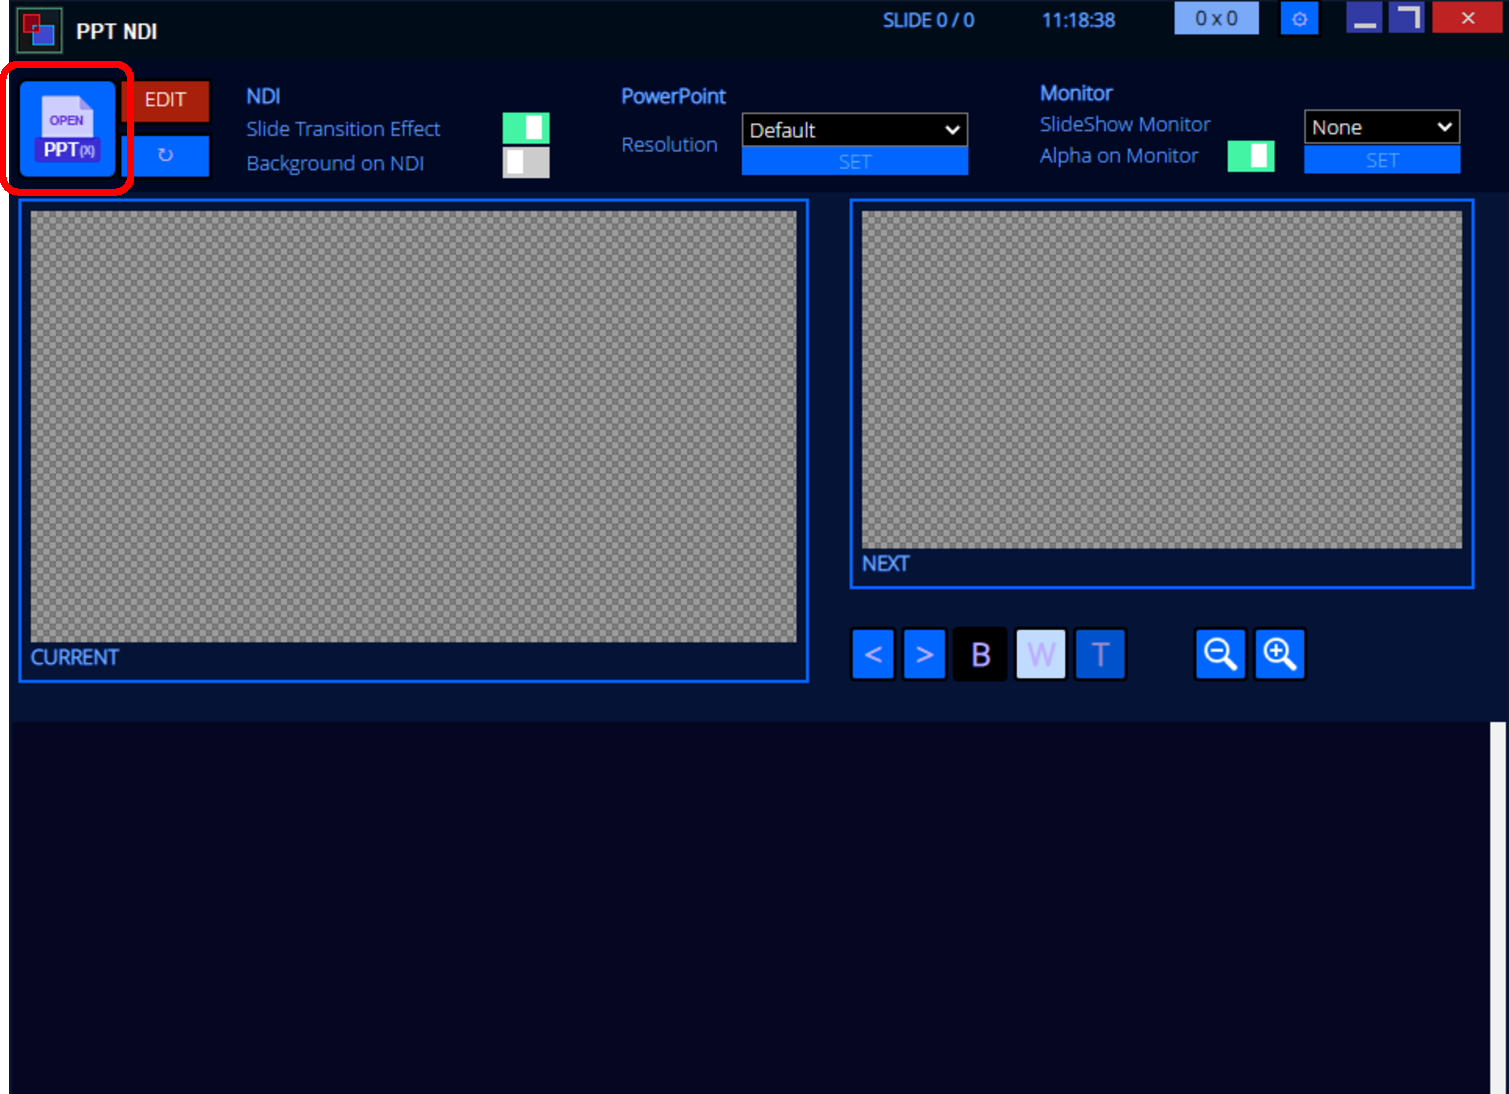
\includegraphics[width=\textwidth]{figures/ppt-ndi}

	\caption{PPT NDI Interface mit \textit{Öffnen}-Button}
	\label{fig:ppt-ndi:interface}
\end{figure}

\begin{figure}[H]
	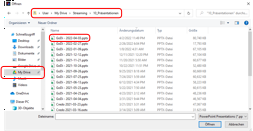
\includegraphics[width=\textwidth]{figures/ppt-ndi-open-dialog}

	\caption{PPT NDI: Präsentation auswählen}
	\label{fig:ppt-ndi:open-dialog}
\end{figure}

\begin{figure}[H]
	\centering
	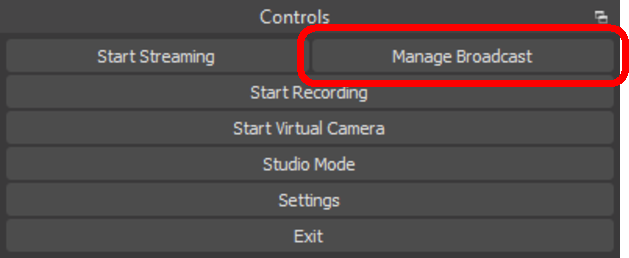
\includegraphics[width=\textwidth]{figures/obs-interface-stream-select}

	\caption{Stream-Select-Fenster in OBS öffnen}
	\label{fig:obs:interface:stream-select}
\end{figure}

\begin{figure}[H]
	\centering
	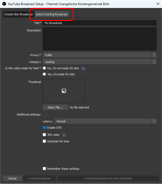
\includegraphics[width=\textwidth]{figures/obs-stream-select}
	
	\caption{Im Stream-Select-Fenster von OBS zu der Streamauflistung wechseln}
	\label{fig:obs:stream-select}
\end{figure}

\begin{figure}[H]
	\centering
	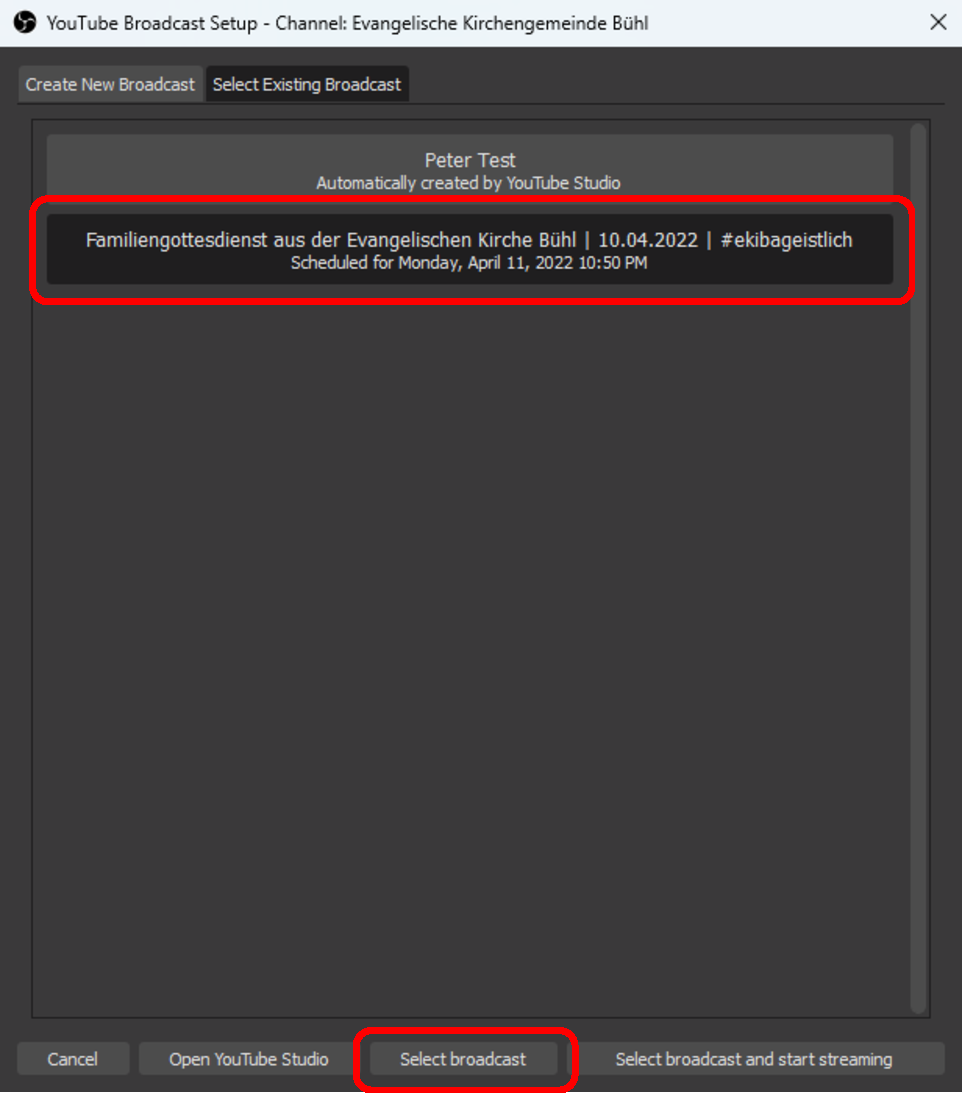
\includegraphics[width=\textwidth]{figures/obs-stream-select-list}
	
	\caption{In der Streamauflistung von OBS den Stream auswählen}
	\label{fig:obs:stream-select-list}
\end{figure}

\begin{figure}[H]
	\centering
	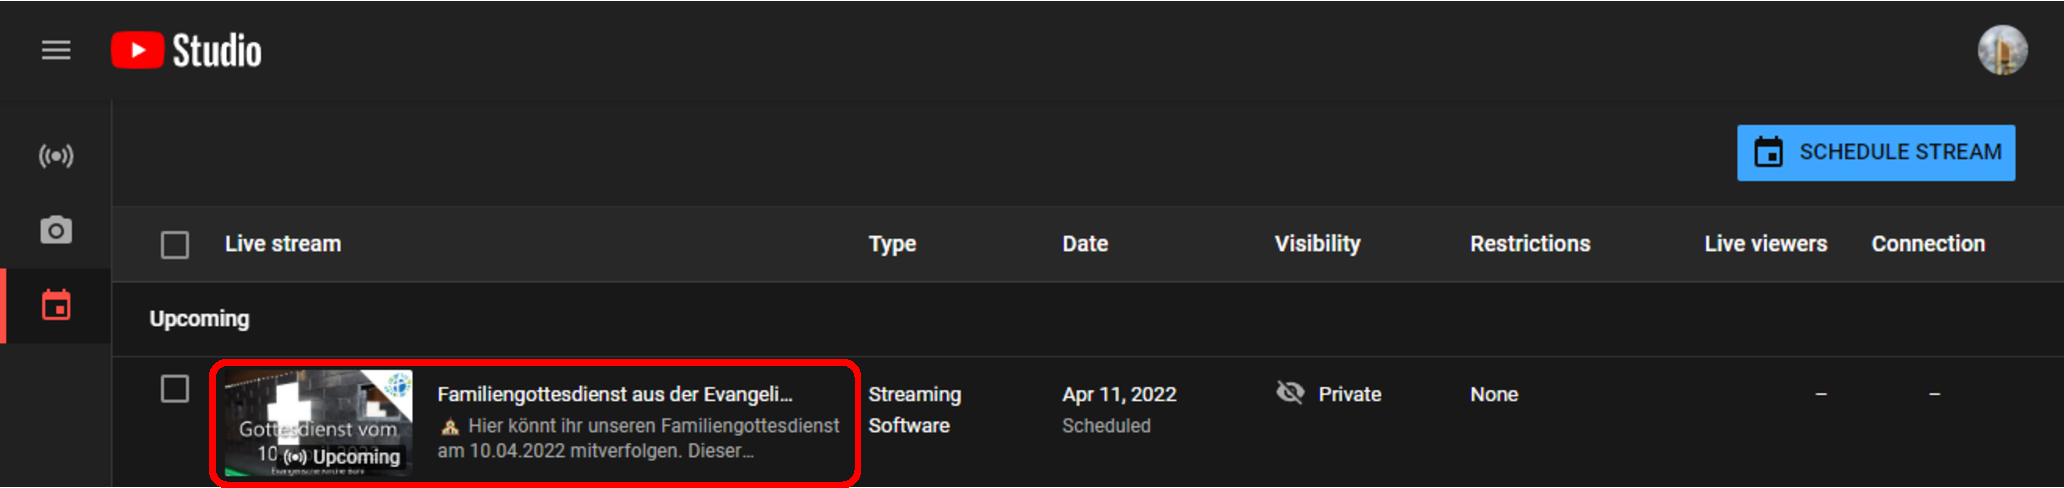
\includegraphics[width=\textwidth]{figures/youtube-livestream-studio}
	
	\caption{Im YouTube-Livestream-Studio den aktuellen Stream auswählen}
	\label{fig:youtube:livestream-studio}
\end{figure}

\begin{figure}[H]
	\centering
	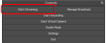
\includegraphics[width=\textwidth]{figures/obs-interface-stream-start}
	
	\caption{In OBS den Livestream starten}
	\label{fig:obs:interface:stream-start}
\end{figure}

\begin{figure}[H]
	\centering
	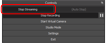
\includegraphics[width=\textwidth]{figures/obs-interface-stream-stop}
	
	\caption{In OBS den Livestream beenden}
	\label{fig:obs:interface:stream-stop}
\end{figure}
\end{document}